\documentclass[12pt]{article}

\usepackage{graphicx}
\usepackage{geometry}
\geometry{
	a4paper,
 	left=24mm,
 	right=24mm,
 	top=30mm,
 	bottom=35mm
}
\usepackage{color}
\definecolor{bluekeywords}{rgb}{0.13,0.13,1}
\definecolor{greencomments}{rgb}{0,0.5,0}
\definecolor{redstrings}{rgb}{0.9,0,0}

\usepackage{listings}
\lstdefinelanguage{FSharp}%
{morekeywords={let, new, match, with, rec, open, module, namespace, type, of, member, % 
and, for, while, true, false, in, do, begin, end, fun, function, return, yield, try, %
mutable, if, then, else, cloud, async, static, use, abstract, interface, inherit, finally },
  otherkeywords={ let!, return!, do!, yield!, use!, var, from, select, where, order, by },
  keywordstyle=\color{bluekeywords},
  sensitive=true,
  basicstyle=\ttfamily,
	breaklines=true,
  xleftmargin=\parindent,
  aboveskip=\bigskipamount,
	tabsize=4,
  morecomment=[l][\color{greencomments}]{///},
  morecomment=[l][\color{greencomments}]{//},
  morecomment=[s][\color{greencomments}]{{(*}{*)}},
  morestring=[b]",
  showstringspaces=false,
  literate={`}{\`}1,
  stringstyle=\color{redstrings},
}
\definecolor{codegreen}{rgb}{0,0.6,0}
\definecolor{codegray}{rgb}{0.5,0.5,0.5}
\definecolor{codepurple}{rgb}{0.58,0,0.82}
\definecolor{backcolour}{rgb}{0.95,0.95,0.92}
\lstdefinestyle{mystyle}{
    backgroundcolor=\color{backcolour},   
    commentstyle=\color{codegreen},
    keywordstyle=\color{magenta},
    numberstyle=\tiny\color{codegray},
    stringstyle=\color{codepurple},
    basicstyle=\footnotesize\ttfamily,
    breakatwhitespace=false,         
    breaklines=true,                 
    captionpos=b,                    
    keepspaces=true,                 
    numbers=left,                    
    numbersep=5pt,                  
    showspaces=false,                
    showstringspaces=false,
    showtabs=false,                  
    tabsize=4
}
\lstset{style=mystyle}
\begin{document}


\begin{center}

{\large F\# Tutorial\\} \vspace{2mm}
\textbf{\LARGE Pipe-Forward Operator}\\
\vspace{1.5mm}
{\Large\emph{\today}}

\end{center}


\section{Syntax, variables, functions}

\subsection{Key concepts: } 

\begin{enumerate}
\item Having a good text editor helps you code much easier.
\item 
\begin{enumerate}
\item Once defined, a variable in F\# cannot change value (unless "mutable" is used)
\item If you need an updated value, create a new one.
\end{enumerate}
\item Different datatypes (e.g. integer and decimal-numbers) do not combine easily.
\item Defining and using functions in F\# is slightly different from math notation/ other languages.
\begin{enumerate}
\item F\# automatically detects the type of the variables (e.g. integer, double, etc.) for a function.
\item The variable types for a function will be enforced.
\end{enumerate}
\end{enumerate}

\subsection{Introduction: } 
\subsubsection{Comments}
You can use double-slash \texttt{//}, triple-slash \texttt{///}, or star-bracket \texttt{(* ...... *)} to make comments.

\begin{lstlisting}[language=FSharp]
// These words are ignored.
/// These words are ignored.
(* These words are ignored. *)
let x = 1
let y = x + 5
\end{lstlisting}

If you are using Visual Studio, you can run the code above by highlighting/selecting the code using your mouse, and press \texttt{ALT + ENTER}, or right-click and select \texttt{Execute in Interactive}.

\vfill

\pagebreak

\subsubsection{Intellisense}
If you are using Visual Studio or Visual Studio Code, you can put your mouse on top of the variable name \texttt{x} or \texttt{y}, and see that it is an \texttt{int} or integer.

This feature will help you identify what is each variable/function, and make coding easier for you. 
\begin{center}
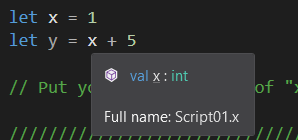
\includegraphics[width=5cm]{pictures/picture01.png}
\end{center}

\subsubsection{Common data types and printing}

Some of the common types in F\# are:
\begin{center}
\begin{tabular}{|c|c|c|}
\hline Keyword & Description & Print in output:
\\ \hline \texttt{int} & Integer & \texttt{\%i}
\\ \hline \texttt{double} or \texttt{float} & Decimal numbers & \texttt{\%f}
\\ \hline \texttt{string} & Words/Sentences & \texttt{\%s}
\\ \hline \texttt{bool} & True/False & \texttt{\%b}
\\ \hline - & Other objects & \texttt{\%A} or \texttt{\%O}
\\ \hline
\end{tabular}
\end{center}

\begin{lstlisting}[language=FSharp]
let name = "John"
let age = 21
let height = 170.5

printfn "My name is: %s" name
// Output:
// My name is: John

printfn "Name: %s. Age: %i. Height: %f." name age height
// Output:
// Name: John. Age: 21. Height: 170.500000

printfn "His height is: %.2f" height
// Output:
// His height is: 170.50
//// Show only two decimal.
\end{lstlisting}
For example, in the second example, inside the string-format, there are \texttt{\%s, \%i, \%f}. And so, we expect a string, integer, and decimal (in that order) after the string-format specification in order to completely print the result to the output console.

\vfill

\pagebreak

\subsubsection{Equality and simple if-else}

The \texttt{let ... = ...} combination is used to assigned a value to a variable. Other than this situation, the equal sign \texttt{=} is used for equality testing. \texttt{=, <>} are used for equality/inequality testing.


\begin{lstlisting}[language=FSharp]
let valueToTest = 20
let isValueEqualToTwenty = (valueToTest = 20)

if isValueEqualToTwenty then
    printfn "Yes, the value is Twenty"
else 
    printfn "No, the value is not Twenty"
// Output: "Yes, the value is Twenty"
///////////////////////////////////////

let inputUserName = "Jack"

if inputUserName = "John" then
    printfn "Welcome back, John"
else 
    printfn "Access denied."
// Output: "Access denied."
\end{lstlisting}

In Java/C++, \texttt{==, !=} are used for comparison, and in Javascript, \texttt{===, !==} are used.

\subsubsection{Immutability}

In F\#, variables are by default immutable/unchangable. Once defined, the value of a variable cannot be changed. You can make a variable changable/mutable using the keyword \texttt{mutable} and symbol \texttt{<-}, but this is \underline{highly discouraged}. (If you use VisualStudio, then the color of the variable name will change color, warning you of potential mutable values)

\begin{center}
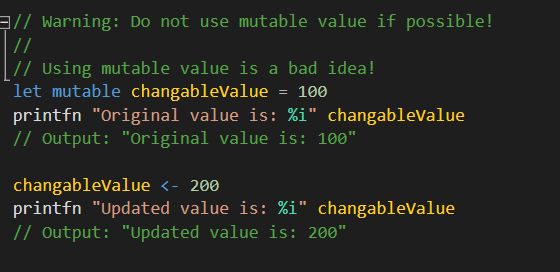
\includegraphics[width=8cm]{pictures/picture02.png}
\end{center}

\vfill

\pagebreak

In addition, if you try to update an immutable/unchangable value using \texttt{<-}, you will get an error. 

\begin{center}
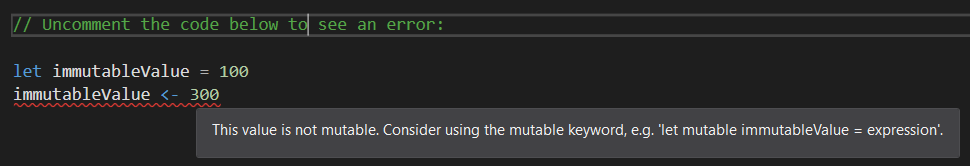
\includegraphics[width=14cm]{pictures/picture03.png}
\end{center}

Why do we recommend immutable/unchangable values: 

Imagine you have a code below, where you have defined a mutable value \texttt{x}, and after thousands of lines of code later, you used \texttt{x}'s value again:

\begin{lstlisting}[language=FSharp]
let mutable x = 100
//
// Thousands of lines of code later......
// You have many lines of code in between......
// It is hard to keep track......
// Have you changed/updated x's value?
// Did you accidentally call any function that modify x?
// Can you guarantee x's value stay unchanged?
// 
//
let y = x + 1
// What is the value of y?
//
// That depends on what happens between y's definition 
// and x's definition.
\end{lstlisting}
\begin{center}
\line(1,0){400}
\end{center}

On the other hand, if \texttt{x} is immutable/unchangable:

\begin{lstlisting}[language=FSharp]
let x = 100
//
// Thousands of lines of code later......
// You have many lines of code in between......
// But because x is immutable/unchangable......
// We can be sure that x stays constant......
// And we can safely conclude that......
//
let y = x + 1
// y = 101
\end{lstlisting}

\pagebreak

\subsubsection{(+) Operator on the same type of variable}

Integers, double, and string support the \texttt{(+)} operation:
\begin{lstlisting}[language=FSharp]

let number1 = 40
let number2 = 55
let addTwoNumbers = number1 + number2

// Remark: "float" and "double" mean the same thing in F#.
let sqrtTwoApprox = 1.414
let piApprox = 3.1415926
let addTwoDecimals = sqrtTwoApprox + piApprox

let sentenceStart = "My school is "
let schoolName = "National University of Singapore"
let combinedSentence = sentenceStart + schoolName
\end{lstlisting}
However, you cannot add an integer with a decimal in F\# directly using \texttt{(+)}, and you cannot add/concatenate a string with a number directly using \texttt{(+)}. If you use VisualStudio, then you may see an error similar to the one below.
\begin{center}
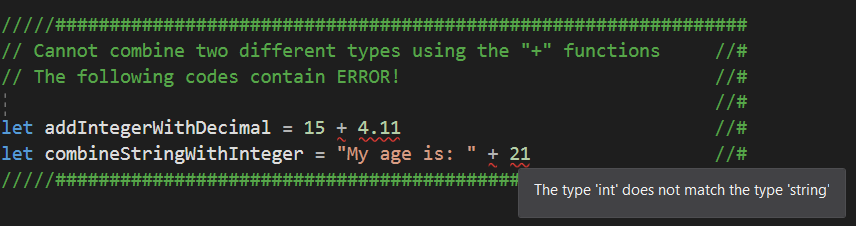
\includegraphics[width=14cm]{pictures/picture04.png}
\end{center}
Furthermore, some functions, like the square root \texttt{sqrt} and math exponent \texttt{(**)} only accepts decimal numbers:

\begin{lstlisting}[language=FSharp]
let sqrtRootOfNine = sqrt 9.0
let twoToPowerOfFive = 2.0 ** 5.0 
\end{lstlisting}
And it will cause error if you use them with integer input instead.
\begin{center}
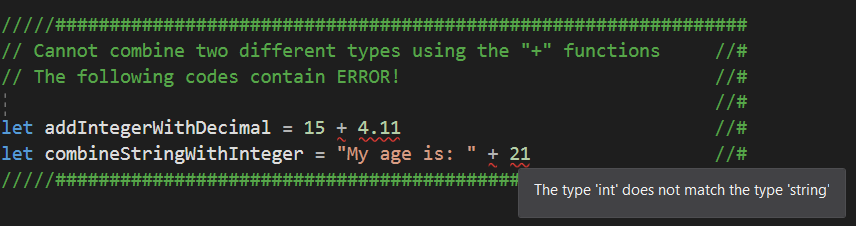
\includegraphics[width=14cm]{pictures/picture04.png}
\end{center}

\pagebreak

\subsubsection{One variable functions}

You can define functions using \texttt{let} followed by the inputs of your function.

\begin{lstlisting}[language=FSharp]
let f x = x + 5

let result1 = f 10
printfn "The result is: %i" result1
// Output: "The result is: 15"

let result2 = f 20
printfn "The result is: %i" result2
// Output: "The result is: 25"
\end{lstlisting}

Notice the following:
\begin{enumerate}
\item To apply the function \texttt{f}, you do not need to use the math notation $f(x)$. You can apply the arguments by separating with a space.
\item If you hover your mouse on top of the function \texttt{f}, you will see that \texttt{f} is a function that accepts only integer \texttt{x} as the argument.
\begin{center}
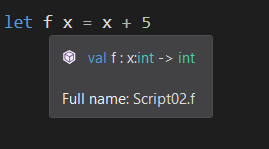
\includegraphics[width=4cm]{pictures/picture06.png}
\end{center}
\begin{enumerate}
\item This is because in the function, \texttt{x} will be added \texttt{(+)} to the integer \texttt{5}. We have seen before that we cannot use the symbol \texttt{(+)} to combine an integer with a decimal number directly. Hence, \texttt{x} has to be of type \texttt{int}.
\item As a consequence, if you try to input a decimal number to the function \texttt{f}, then it will fail:
\begin{center}
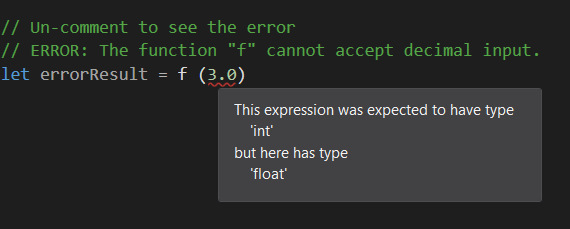
\includegraphics[width=9cm]{pictures/picture07.png}
\end{center}
\end{enumerate}
\item As mentioned, F\# automatically inferred that \texttt{x} is an integer. This is different from other languages (e.g. Java, C++) that needs you to specify the type of the variable (is it an integer? double? etc.)
 
So, you can spend less time on the tiny details (e.g. what is the variable type), and focus more on the correctness of your program.
\end{enumerate}

\pagebreak

Similarly, the following function accepts decimals/double only.

\begin{lstlisting}[language=FSharp]
let DiscountBy20Percent originalPrice = originalPrice * 0.8

let discountedPrice = DiscountBy20Percent 399.99
printfn "The new price is: %.2f" discountedPrice
// Output: "The new price is: 319.99"

let anotherDiscount = DiscountBy20Percent discountedPrice
printfn "The new price is: %.2f" anotherDiscount
// Output: "The new price is: 255.99"
\end{lstlisting}
Remark: The \texttt{\%.2f} is for formatting purposes when printing result, 2 decimals.

Here, if you try to put input an integer value to this function, then you will see an error:
\begin{center}
INPUT ERROR PICTURE HERE!
\end{center}

And in order to use the function on integer values, you need to convert it to decimals using \texttt{double} or \texttt{float} function/keyword.

\begin{lstlisting}[language=FSharp]
let convertedPrice = double 100
let decimalResult = DiscountBy20Percent convertedPrice
printfn "The new price is: %.2f" decimalResult
// Output: "The new price is: 80.00"
\end{lstlisting}
\begin{center}
\line(1,0){400}
\end{center}
Similarly, the following function accepts strings only.
\begin{lstlisting}[language=FSharp]
// Define a function for string.
let AddGreeting name =
    "Hello " + name

let greeting1 = AddGreeting "John"
printfn "The modified sentence is: %s" greeting1
// Output: "The modified sentence is: Hello John"

let greeting2 = AddGreeting "Mary"
printfn "The modified sentence is: %s" greeting2
// Output: "The modified sentence is: Hello Mary"
\end{lstlisting}
And it will cause error if you try to input an integer value to this function:
\begin{center}
INPUT ERROR PICTURE HERE!
\end{center}
\pagebreak
Exercise: Write a function that calculates the area of a circle of radius $r$. 



\begin{lstlisting}[language=FSharp]
let CircleArea r =
     //
     // ... INSERT YOUR CODE HERE ...
     // Hint: Use    "System.Math.PI"
\end{lstlisting}

\subsubsection{Two variable functions}
You can define a function that takes in two variables:
\begin{lstlisting}[language=FSharp]
let g x y = 3 * x + y

let result3 = g 3 1
printfn "The result is: %i" result3
// Output: "The result is: 10"

let result4 = g 10 2
printfn "The result is: %i" result4
// Output: "The result is: 32"
\end{lstlisting}
Notice the following:
\begin{enumerate}
\item To apply the function \texttt{g}, you do not need to use the math notation $g(x,y)$ with brackets and commas. This is different from other programming languages (e.g. Java, C++). You can apply the arguments by separating with a space.
\item If you hover your mouse on top of \texttt{g}, as seen in this picture:
\begin{center}
INPUT PICTURE HERE!
\end{center}
You will see that the variables \texttt{x, y} need to be integers.
\begin{enumerate}
\item This is because in the function, \texttt{x} will be multiplied with \texttt{3}, and then later added with \texttt{y}. As seen before, the addition and multiplication symbol \texttt{(+), (*)} only combined numbers of the same type (integers with integers, double with double)
\item As a consequence, if you input decimals into the function, it will fail:
\begin{center}
INPUT PICTURE HERE!
\end{center}
\end{enumerate}
\item Again, you can spend less time typing out the details (i.e. what are the types of \texttt{x, y}? Integer? Double?) and focus more on making your program/algorithm works, and make yourself more productive (compared to other programming languages)
\end{enumerate}

\pagebreak

Similarly, the following function accepts two decimal numbers:
\begin{lstlisting}[language=FSharp]
let CalculateNewBalance interestRate principal  = 
    principal * (1.0 + interestRate)

let balance1 = CalculateNewBalance 0.05 100000.00 
printfn "The new balance is: %f" balance1
// Output: "The new balance is: 105000.00"

let balance2 = CalculateNewBalance 0.03 5000.00 
printfn "The new balance is: %f" balance2
// Output: "The new balance is: 5150.00"
\end{lstlisting}

And it will cause error if you try to change one of the input into integer.
\begin{center}
INPUT PICTURE HERE!
\end{center}

\subsubsection{Multivariable functions}
\begin{lstlisting}[language=FSharp]
let h x y z = 3 * x + 4 * y + 5 * z

// 3*3 + 4*4 + 5*5 = 50
let result5 = h 3 4 5
printfn "The result is: %i" result5
// Output: "The result is: 50"

// 3*1 + 4*1 + 5*1 = 12
let result6 = h 1 1 1
printfn "The result is: %i" result6
// Output: "The result is: 12"
\end{lstlisting}

\subsubsection{Default integers for +, *}
If you use \texttt{(+), (*)} with no other information available in your function (e.g. an appearance of a decimal, string, etc.), then F\# will assume the function variables as integers.
\begin{lstlisting}[language=FSharp]
let AddThree x y z = x + y + z
let addThreeResult = AddThree 5 6 7
\end{lstlisting}
If you hover your mouse on top of \texttt{AddThree}, the you see that all the inputs are inferred to be integers.

If you want this function to work for decimals, then you will need to annotate/manually add in the type for one of the variables:
\begin{lstlisting}[language=FSharp]
let AddThreeCustom (x:double) y z = x + y + z
\end{lstlisting}
Here, we are explicitly saying that \texttt{x} is a double. And since \texttt{y, z} interacts with \texttt{x} using \texttt{(+)}, we can infer that \texttt{y, z} are also doubles (and we do not need to explicitly label them as decimal/doubles)

\pagebreak




\begin{lstlisting}[language=FSharp]
let DiscountBy20Percent originalPrice = originalPrice * 0.8
// Output: "The new price is: 255.99"
\end{lstlisting}

\begin{lstlisting}[language=FSharp]
let DiscountBy20Percent originalPrice = originalPrice * 0.8
// Output: "The new price is: 255.99"
\end{lstlisting}


\pagebreak

\appendix
\section{Appendix}

\subsection{Optional Topics}
\subsubsection{inline functions}
On some occasion, if you need to use the same function on different type which supports \texttt{(*)}, then you can use the \texttt{inline} keyword.
\begin{lstlisting}[language=FSharp]
let inline Product x y = x * y

let multiply2Int = Product 2 3
printfn "Multiply the two numbers gives: %i" multiply2Int
// Output: "Multiply the two numbers gives: 6"

let multiply2Double = Product 3.0 4.0
printfn "Multiply the two numbers gives: %f" multiply2Double
// Output: "Multiply the two numbers gives: 12.000000"
\end{lstlisting}
However, not every datatype supports multiplication \texttt{(*)}
\begin{center}
INPUT PICTURE HERE!
\end{center}
\begin{center}
\line(1,0){400}
\end{center}
Similarly, we can do this:
\begin{lstlisting}[language=FSharp]
let inline CustomAdd x y z = x + y + z
let add3IntegerResult = CustomAdd 4 5 6
printfn "Adding the three integers give: %i" add3IntegerResult
// Output: "Adding the three integers give: 15"

let add3StringResult = CustomAdd "John " "F." " Kennedy"
printfn "Concatenate the three strings give: %s" add3StringResult
// Output:
// "Concatenate the three strings give: John F. Kennedy"

let add3DecimalResult = CustomAdd 10.3 10.2 10.1
printfn "Adding the three decimals give: %f" add3DecimalResult
// Output: "Adding the three decimals give: 30.600000"
\end{lstlisting}
However, not every datatype supports addition \texttt{(+)}
\begin{center}
INPUT PICTURE HERE!
\end{center}

\end{document}